\section{前期准备}
使用虚拟机运行raven,首先需要准备一台计算机,在计算机中安装虚拟机软件,再下载虚拟机备份文件。
\subsection{安装虚拟机}
在\href{https://www.vmware.com/products/workstation-player/workstation-player-evaluation.html}{VMware官网}下载VMware Workstation 16.0 Player,如图\ref{VM下载界面}所示。
\begin{figure}[h]
    \centering
    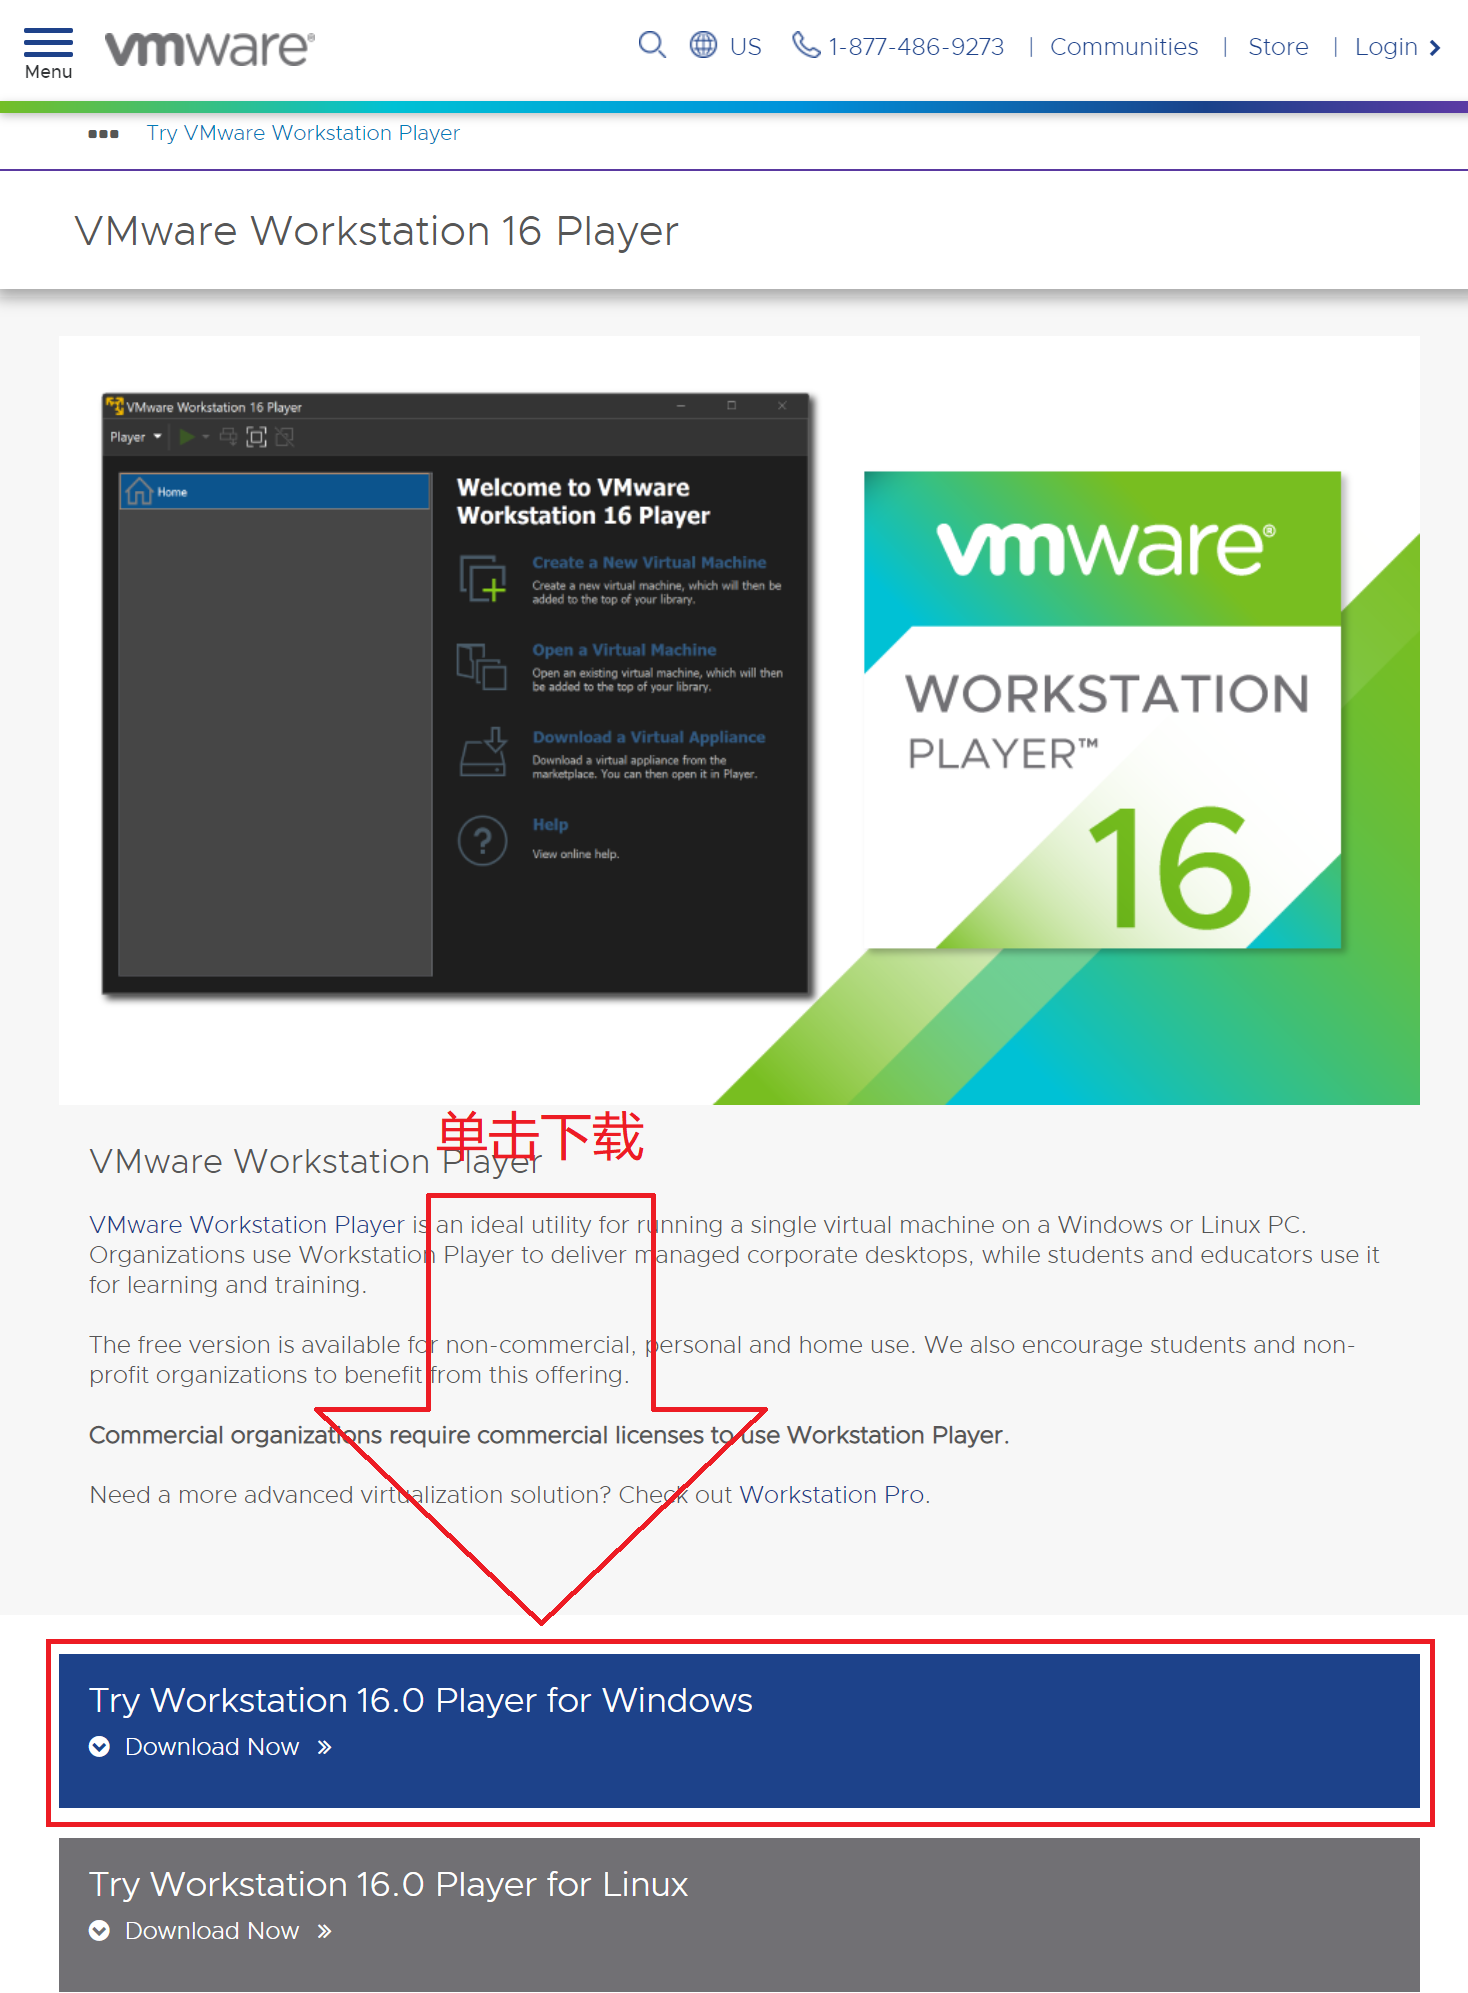
\includegraphics[width=0.75\textwidth]{www.vmware.com_products_workstation-player_workstation-player-evaluation.html.png}
    \caption{VM下载界面}
    \label{VM下载界面}
\end{figure}

下载后按其安装指导安装VMware!

\subsection{下载虚拟机备份文件}
从\href{https://hrbeueducn-my.sharepoint.com/:u:/g/personal/6ming_hrbeu_edu_cn/EeUGCVn3UFVIooQBe_4KA84B91BWppg__eVfWB9nZlAKkA?e=g2146y}{网盘}下载windows10虚拟机备份文件压缩包,如图\ref{网盘}所示:
\begin{figure}[ht]
    \centering
    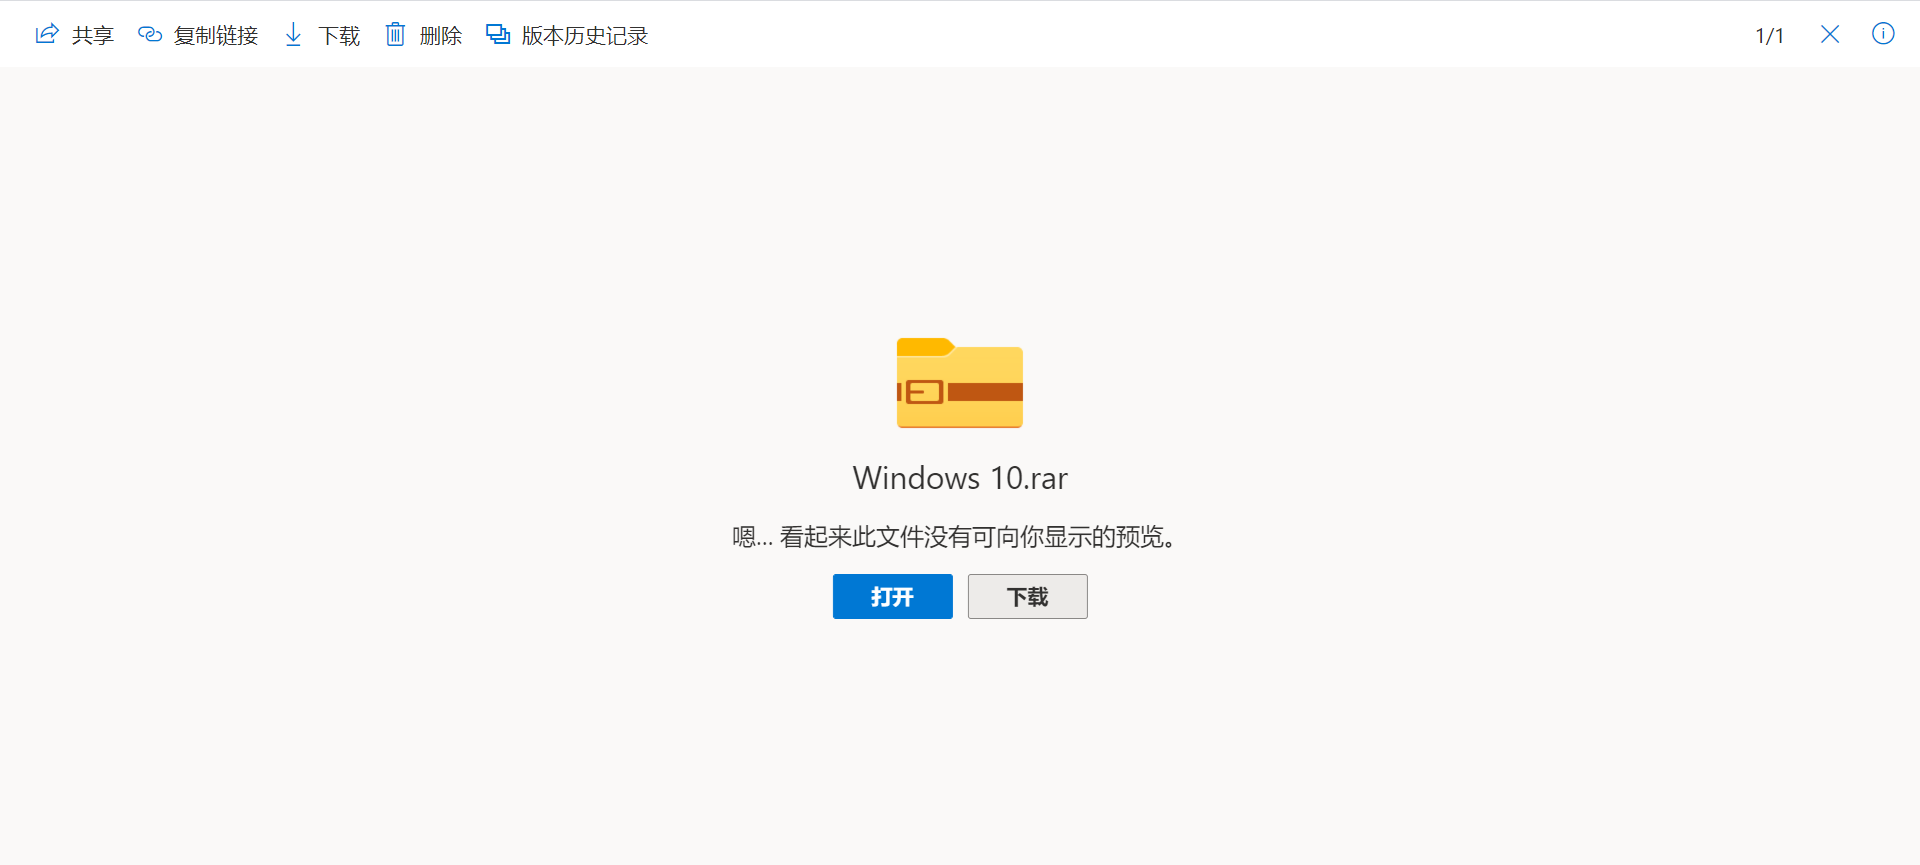
\includegraphics[width=0.9\textwidth]{Windows10虚拟文件压缩包.png}
    \caption{网盘}
    \label{网盘}
\end{figure}

从网盘下载windows.rar文件,解压,后得到解压文件,如\ref{解压后文件}所示:
\begin{figure}[ht]
    \centering
    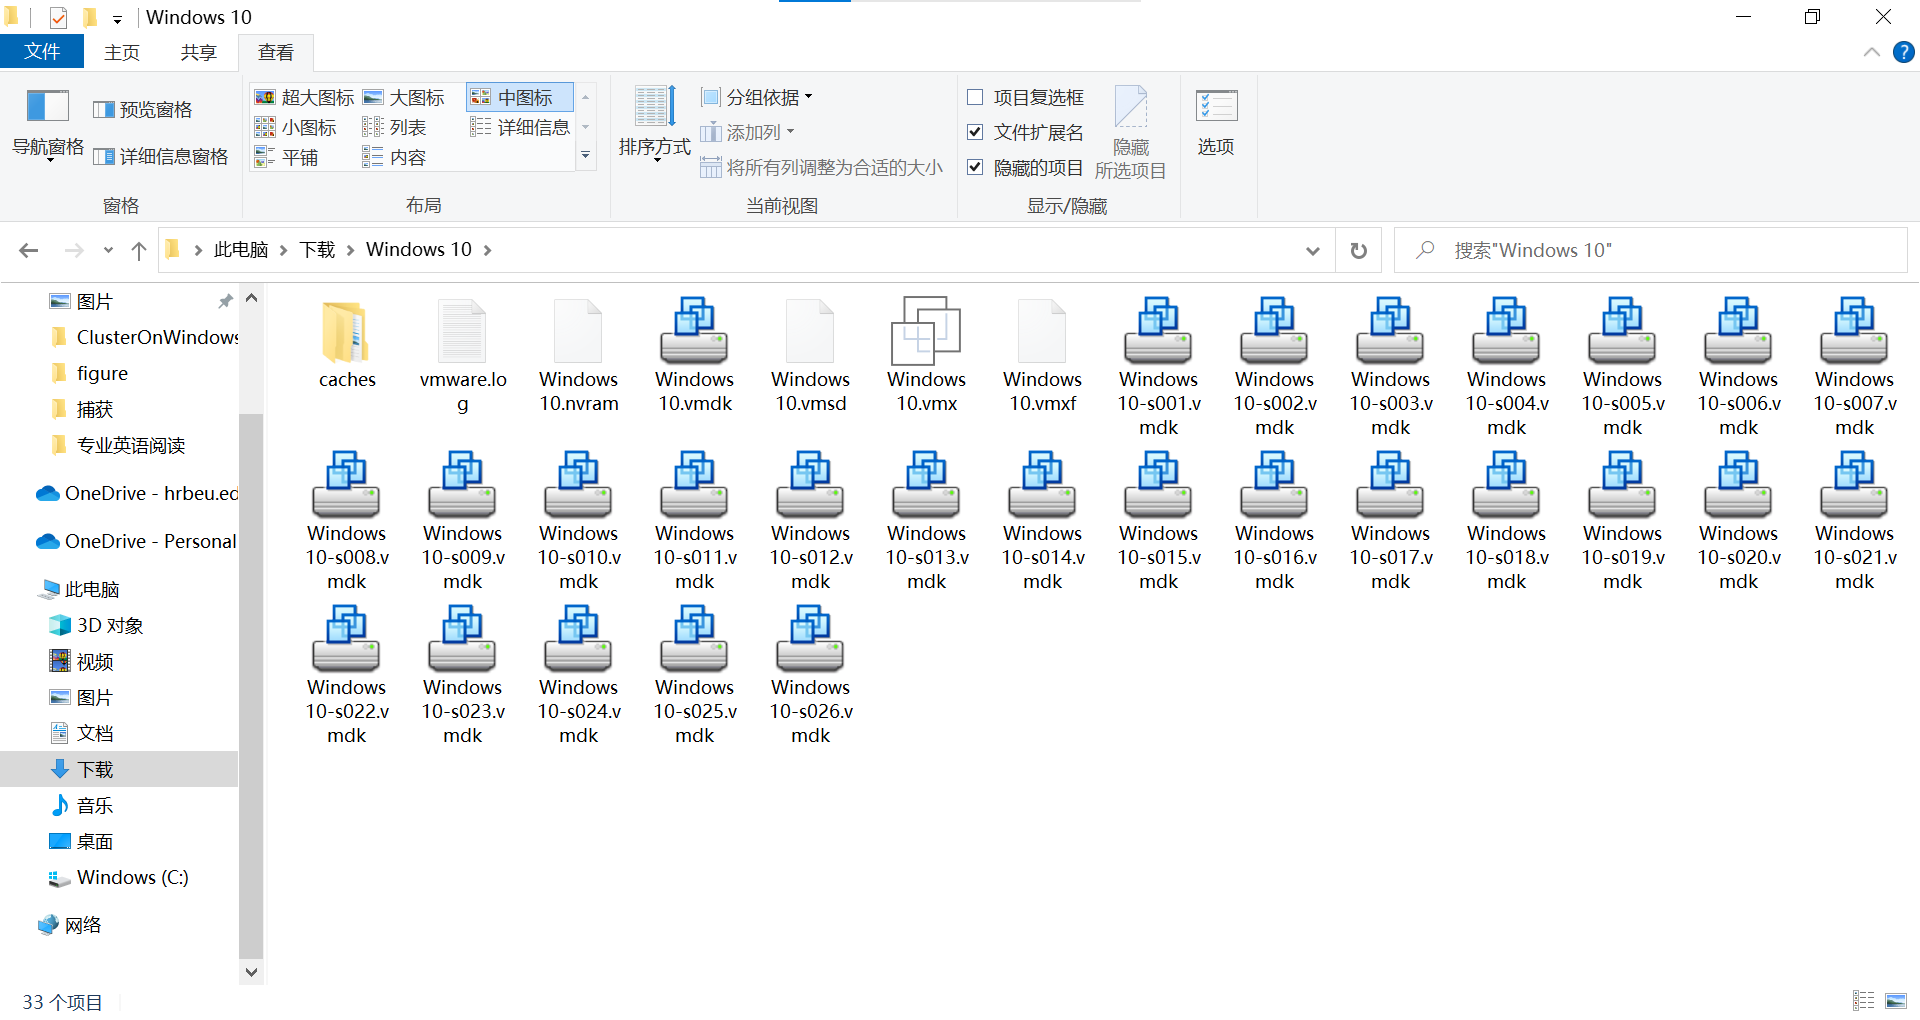
\includegraphics[width=0.9\textwidth]{解压后文件.png}
    \caption{解压后文件}
    \label{解压后文件}
\end{figure}

建议解压后将其移动到虚拟机目录下。

\section{建立虚拟机}
打开VMware,点击打开虚拟机,如图\ref{打开虚拟机}所示:
\begin{figure}[ht]
    \centering
    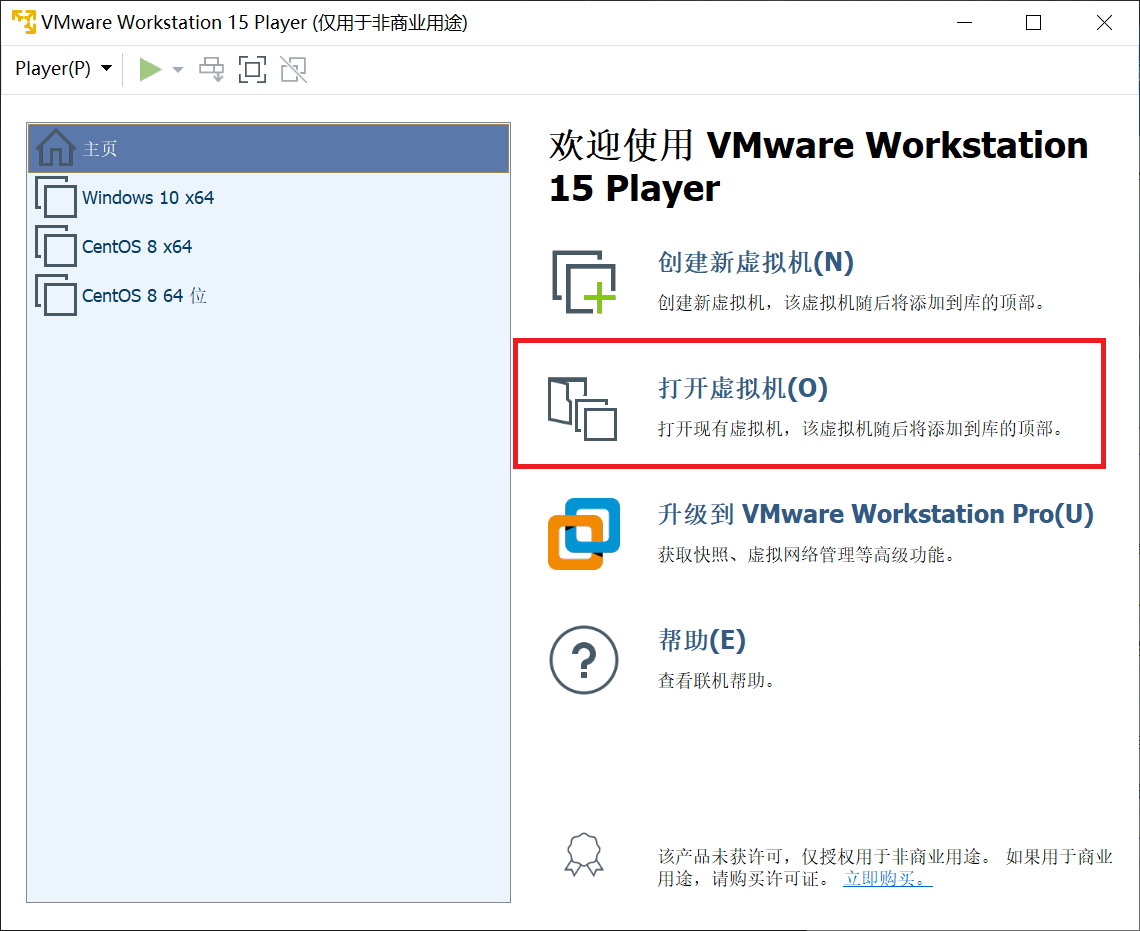
\includegraphics[width=0.56\textwidth]{打开现有虚拟机.png}
    \caption{打开虚拟机}
    \label{打开虚拟机}
\end{figure}

选择$ Windows 10.vmx $,点击“打开”,如图\ref{选择虚拟文件}所示:
\begin{figure}[ht]
    \centering
    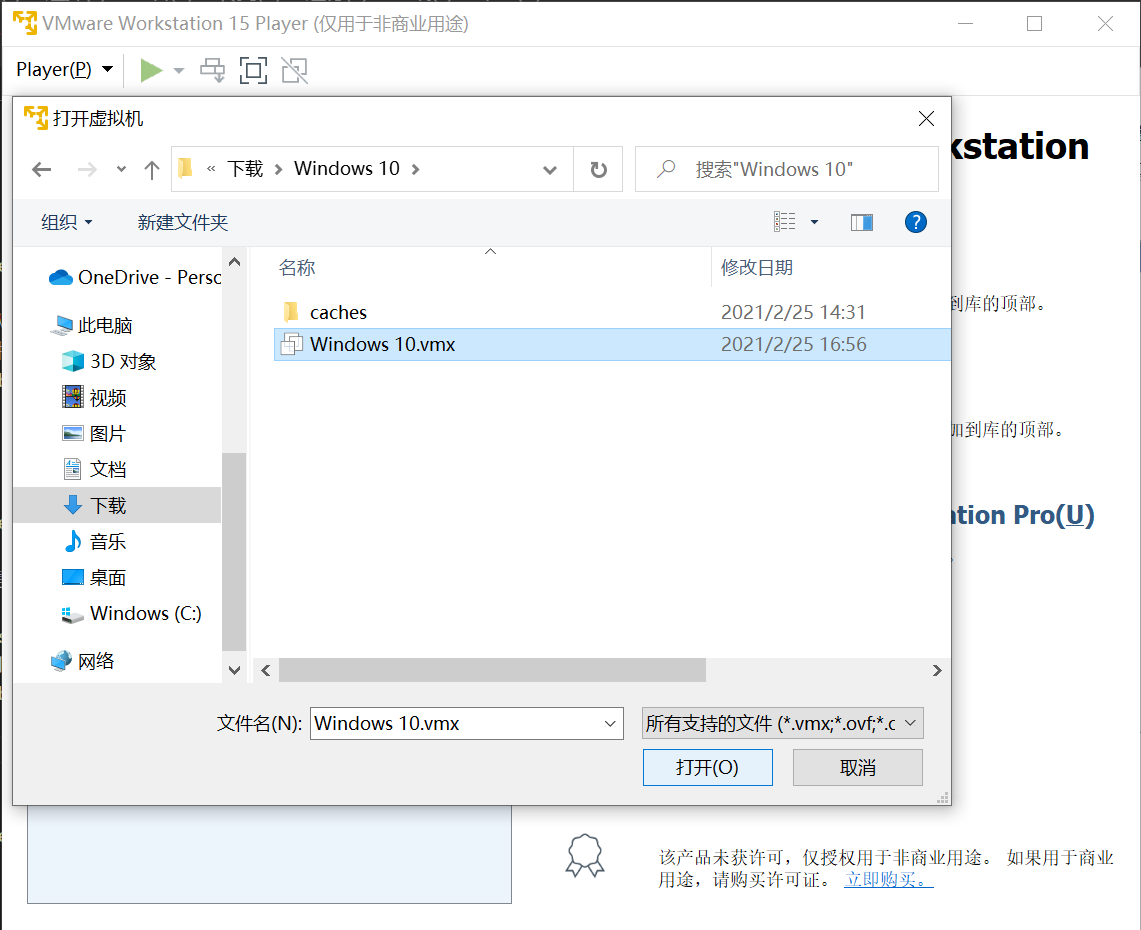
\includegraphics[width=0.57\textwidth]{选择虚拟备份文件.png}
    \caption{选择虚拟文件}
    \label{选择虚拟文件}
\end{figure}

点击“播放虚拟机”,如图\ref{播放虚拟机}所示:
\begin{figure}[ht]
    \centering
    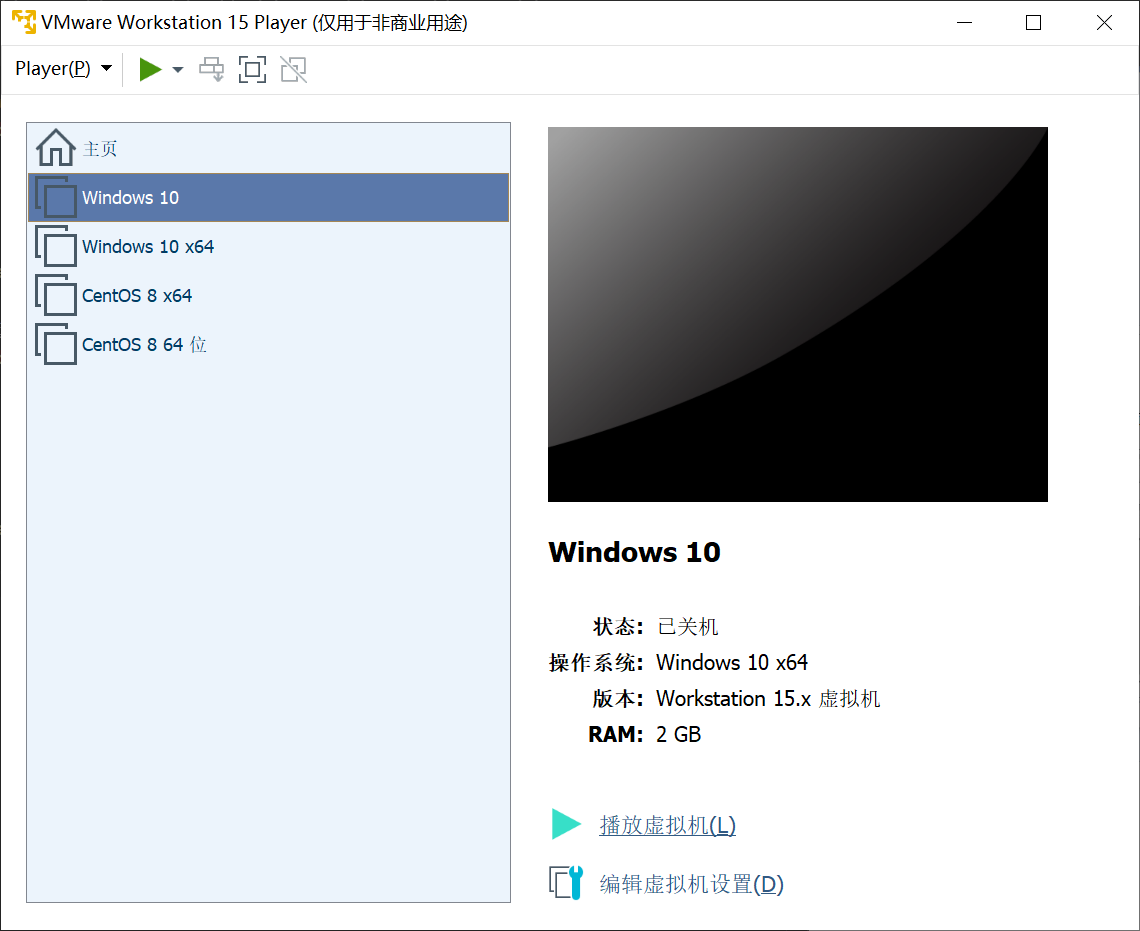
\includegraphics[width=0.7\textwidth]{播放虚拟机.png}
    \caption{播放虚拟机}
    \label{播放虚拟机}
\end{figure}

登录虚拟机后,便可在桌面上打开raven文件夹,如图\ref{虚拟机界面}所示:
\begin{figure}[htpb]
    \centering
    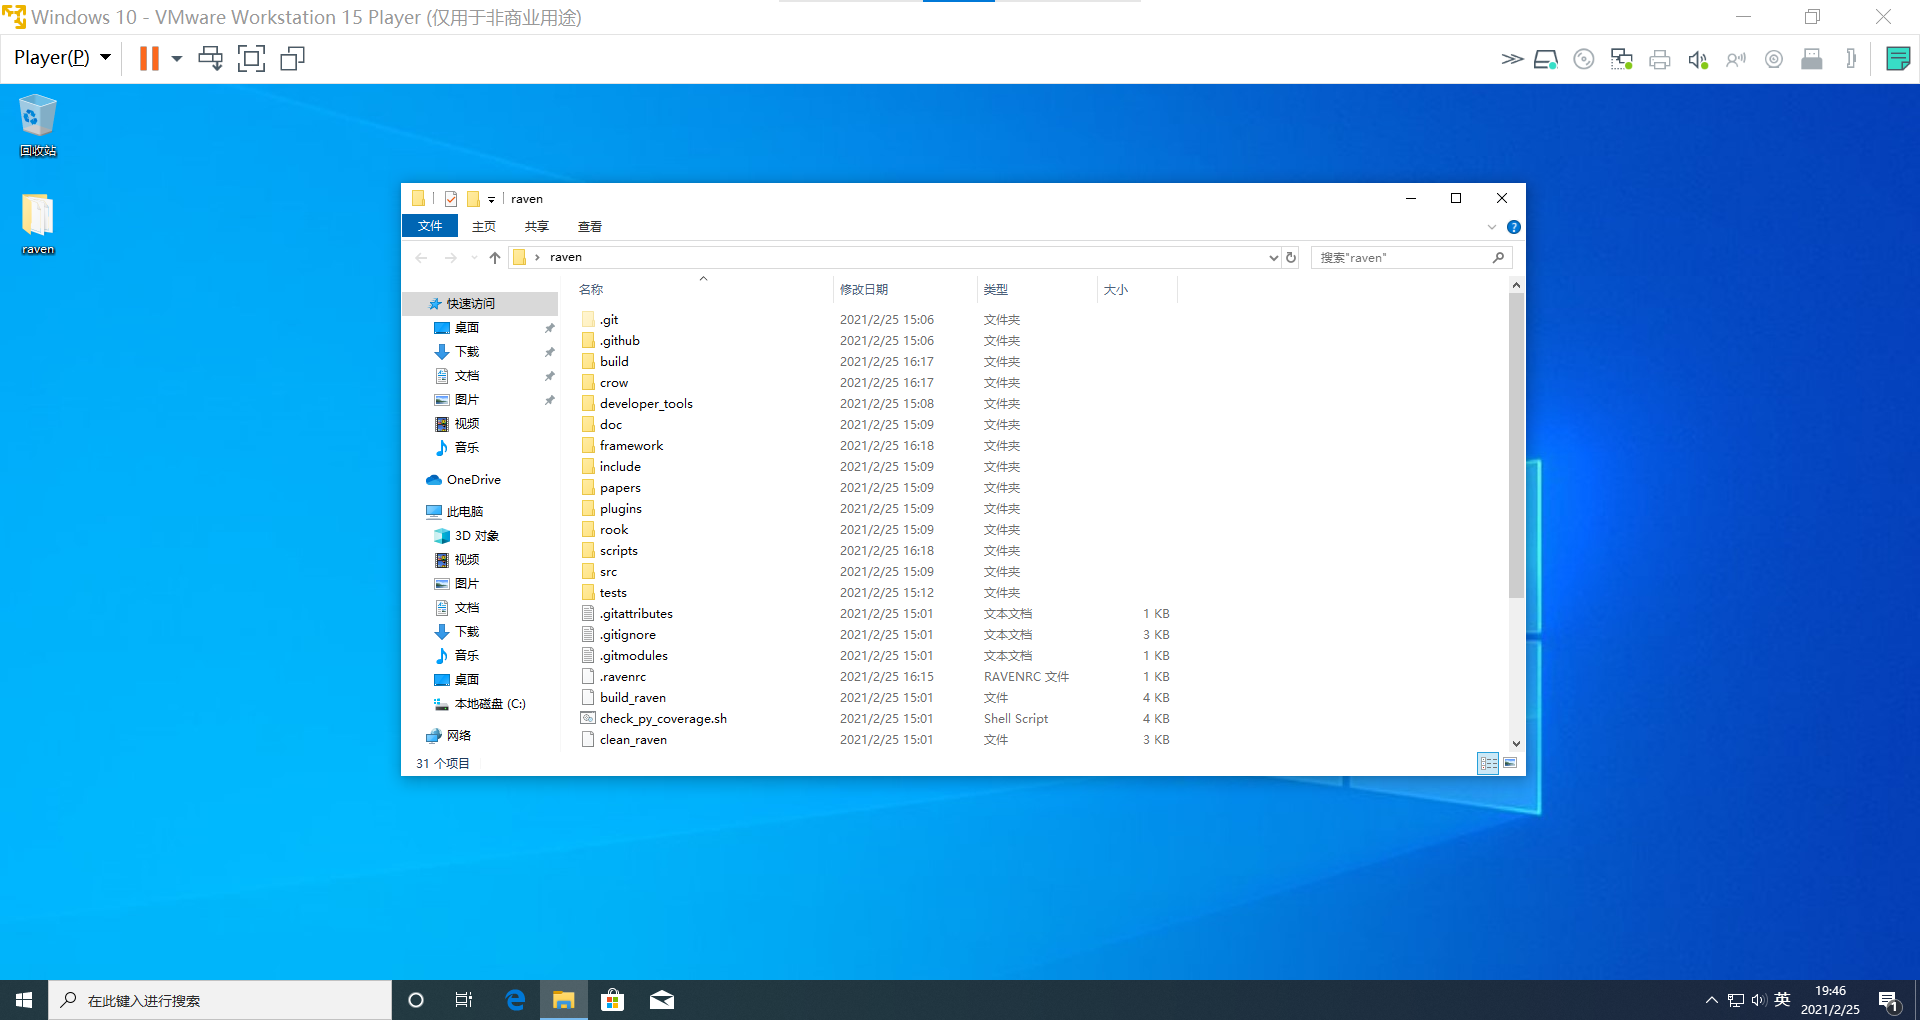
\includegraphics[width=1.0\textwidth]{虚拟机界面.png}
    \caption{虚拟机界面}
    \label{虚拟机界面}
\end{figure}

\section{运行raven}

在raven文件夹中,右键选择"Git Bash Here",如图\ref{选择Git Bash}所示。
\begin{figure}
    \centering
    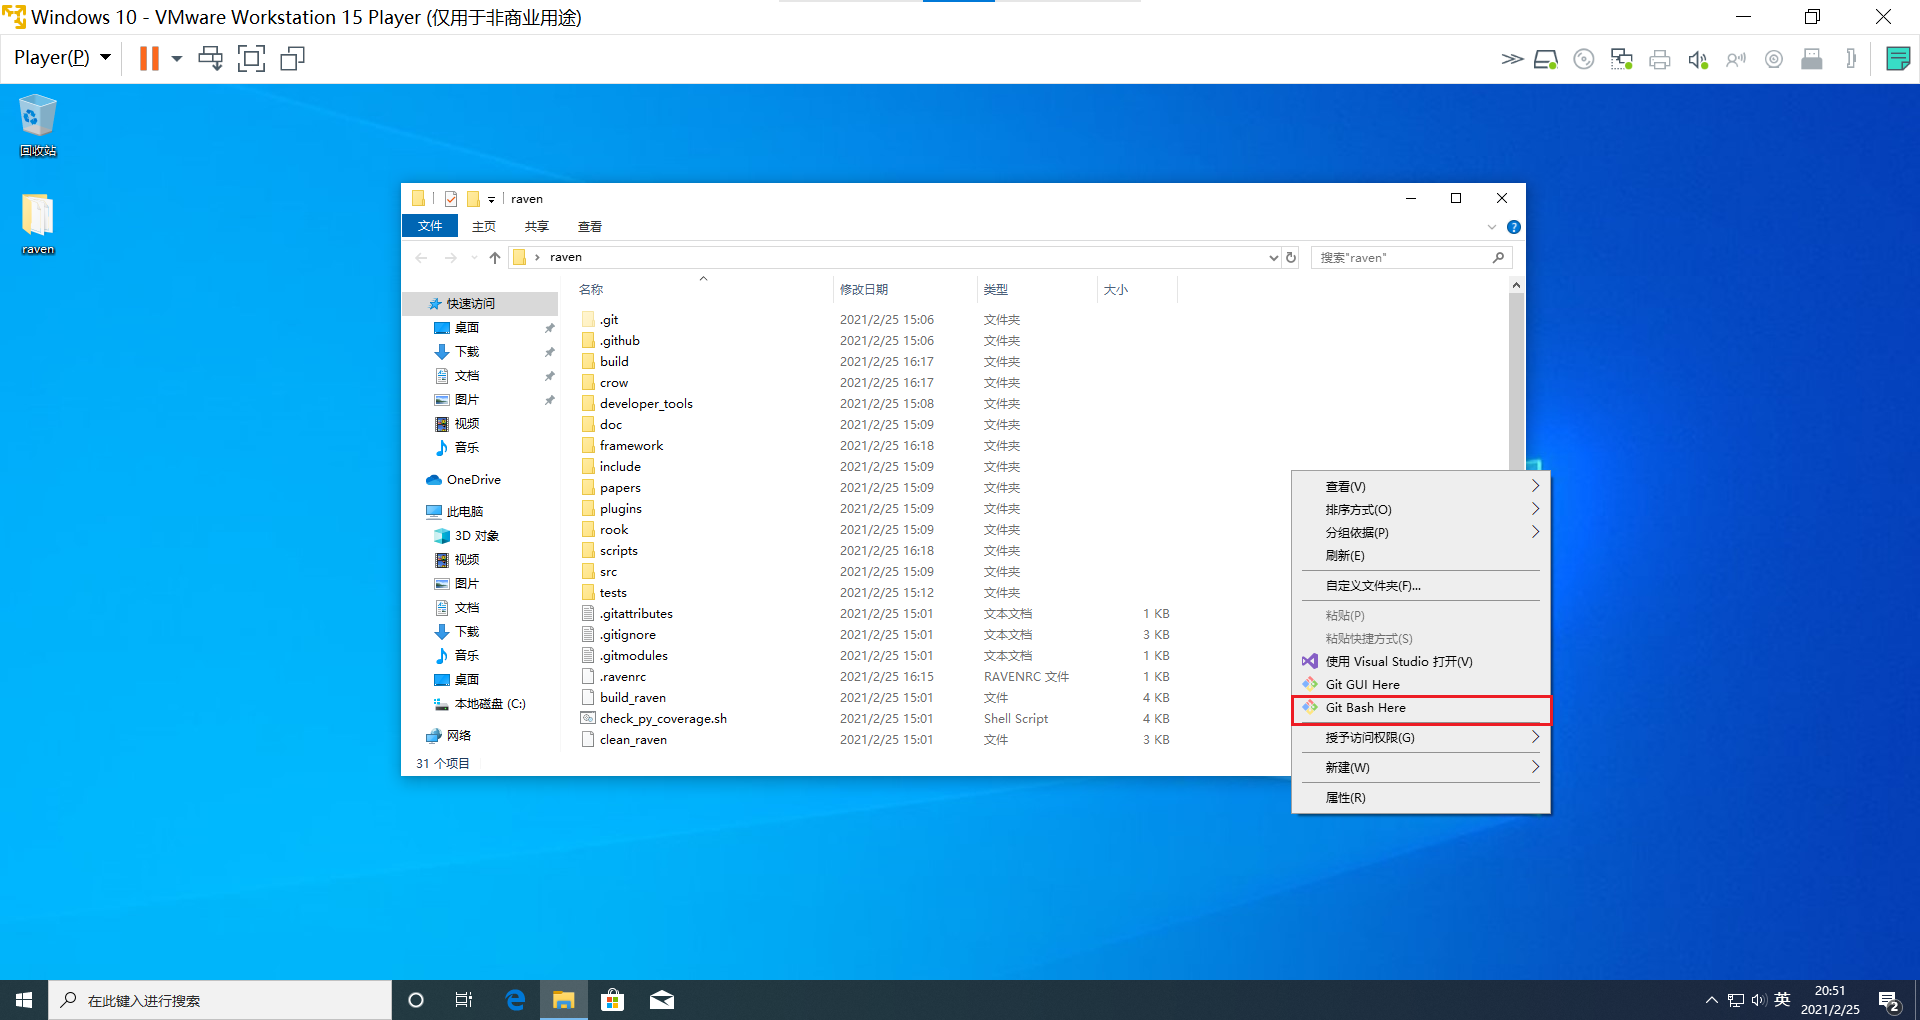
\includegraphics[width=1.0\textwidth]{Bash Here.png}
    \caption{选择Git Bash}
    \label{选择Git Bash}
\end{figure}

输入命令行指令$ ./raven\_framework RunFile $运行raven,如图\ref{命令行运行raven}所示。
\begin{figure}[ht]
    \centering
    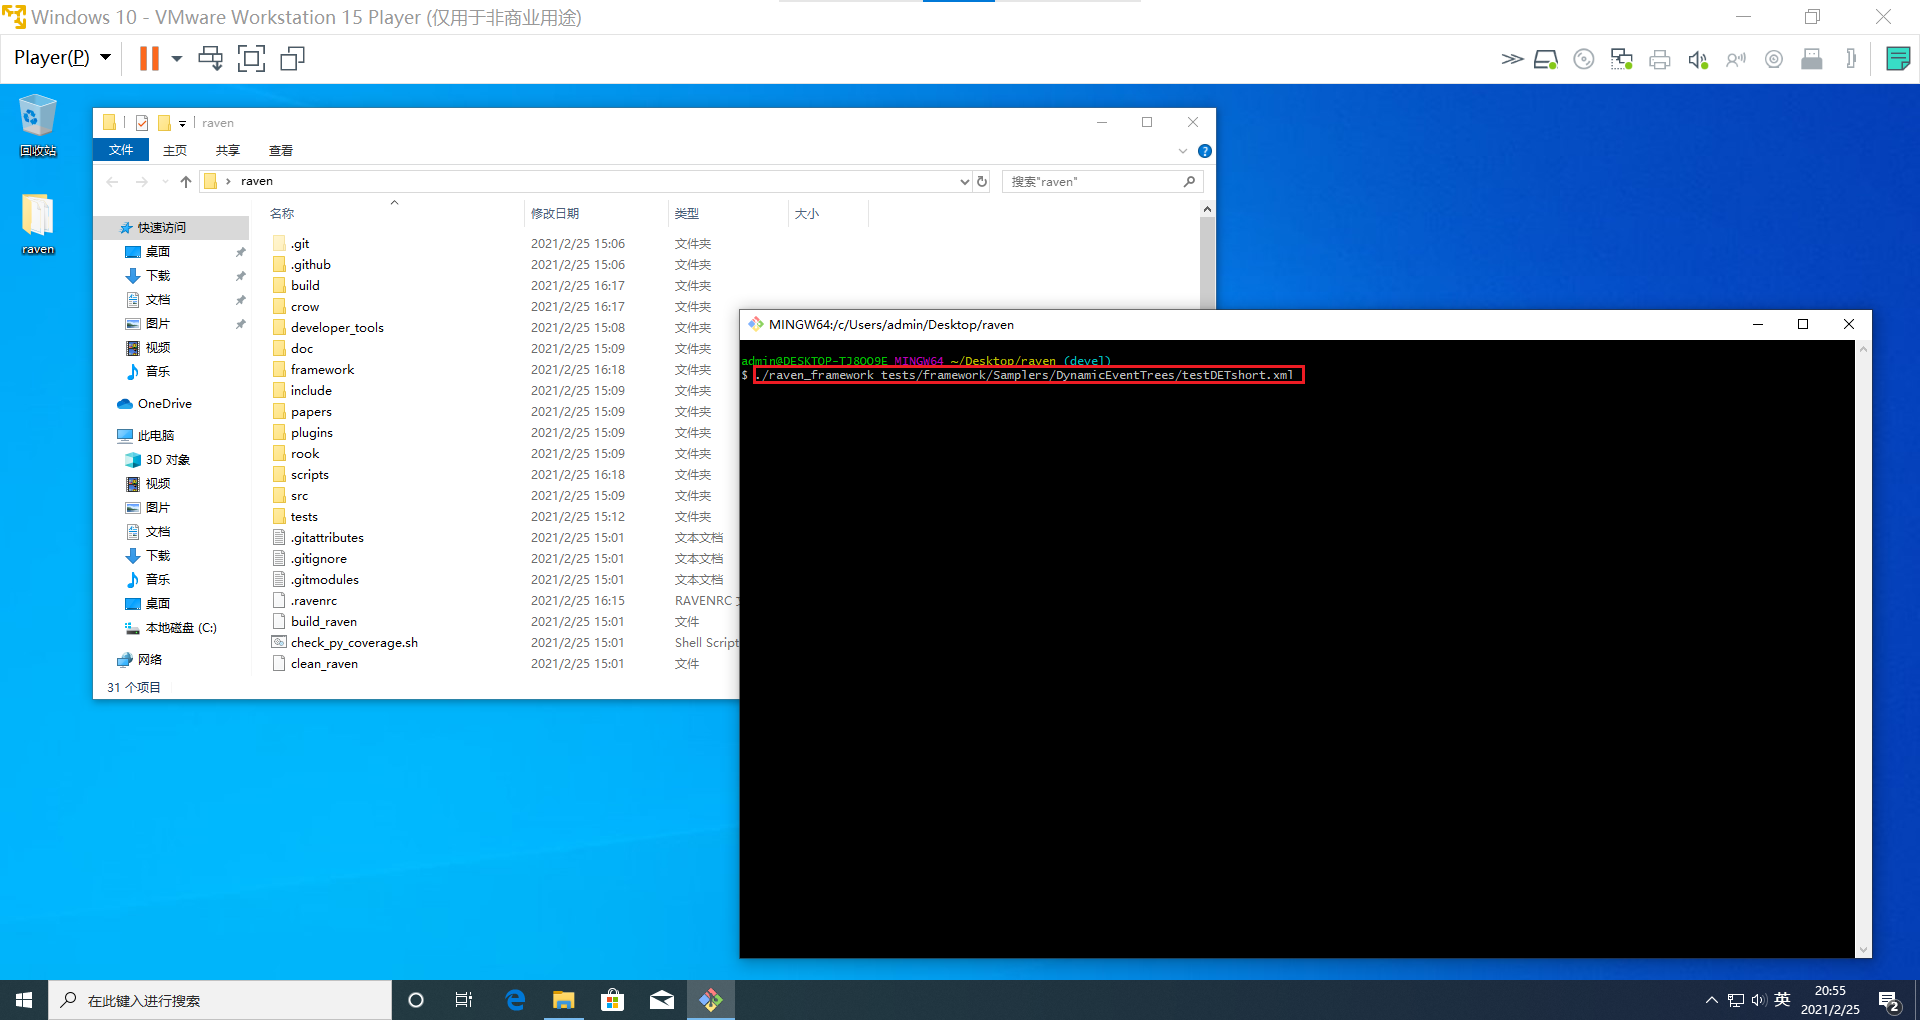
\includegraphics[width=1.0\textwidth]{运行raven.png}
    \caption{命令行运行raven}
    \label{命令行运行raven}
\end{figure}

运行完成后,屏幕输出$ Run Complete! $,则表示运行成功,如图\ref{RAVEN运行结果}所示。
\begin{figure}[ht]
    \centering
    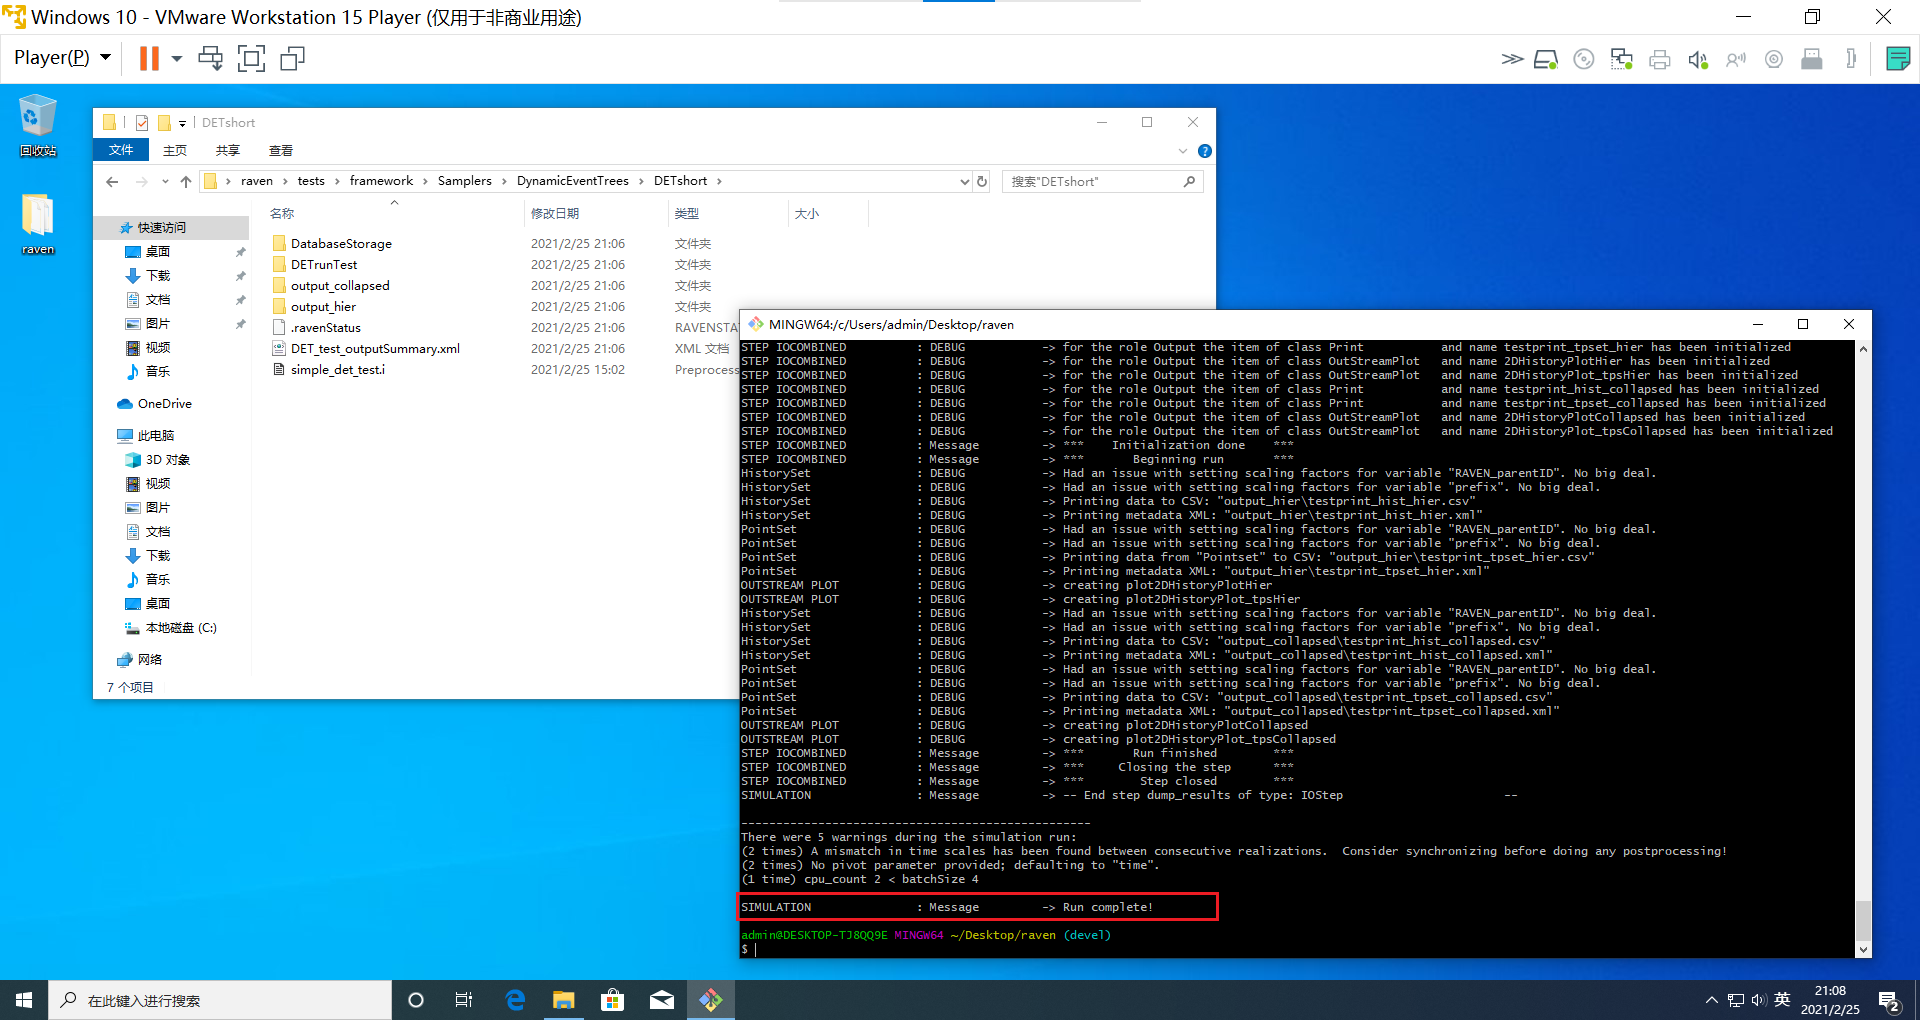
\includegraphics[width=1.0\textwidth]{运行结果.png}
    \caption{RAVEN运行结果}
    \label{RAVEN运行结果}
\end{figure}